\documentclass[prx,12pt]{revtex4-2}
\usepackage{amsmath}
\usepackage{amssymb}
\usepackage{graphicx}
\usepackage{color}
\usepackage{mathrsfs}
\usepackage{enumerate}
\usepackage{epigraph}
\usepackage{framed}
\usepackage[pdfborder={0 0 0},colorlinks=true,linkcolor=blue,urlcolor=blue]{hyperref}

\def\ket#1{\left|#1\right\rangle}
\def\bra#1{\left\langle#1\right|}
\def\braket#1{\left\langle#1\right\rangle}
\def\hvbox[#1]#2{\,\boxed{\scalebox{0.7}{$\,#1$}|\scalebox{0.7}{$#2\,$}}}

\usepackage{fancyhdr}
\fancyhf{}
\lhead{\tiny Y.~D.~Chong}
\rhead{\scriptsize Ch.~3: Quantum Entanglement $|$ Graduate Quantum Mechanics}
\lfoot{}
\rfoot{\thepage}
\pagestyle{fancy}

\setlength{\parindent}{14pt}
\setlength{\fboxsep}{0.01\fboxsep}
\renewcommand{\theequation}{3.\arabic{equation}}

\renewcommand{\baselinestretch}{1.0}
\setlength{\parskip}{0.04in}

\def\thesection{3.\arabic{section}}
\def\thesubsection{\thesection.\arabic{subsection}}

\makeatletter
\renewcommand{\p@subsection}{}
\renewcommand{\p@subsubsection}{}
\makeatother

\begin{document}
\setcounter{page}{36}

\begin{center}
{\Large \textbf{Chapter 3: Quantum Entanglement}}
\end{center}

\epigraph{They don't think it be like it is, \\but it do.}{Oscar Gamble}

\section{Quantum states of multi-particle systems}

So far, we have studied quantum mechanical systems consisting of
single particles; the next important step is to consider systems of
multiple particles.  As we shall see, applying the postulates of
quantum mechanics to multi-particle systems leads to many important
and counterintuitive phenomena, such as \textbf{quantum entanglement}.

\subsection{Tensor products}
\label{sec:tensorprod}

Suppose we have two quantum objects, $A$ and $B$.  According to
quantum mechanics, $A$ is associated with some Hilbert space
$\mathscr{H}_A$ (i.e., every state of A is a vector in that space),
and $B$ is similarly associated with a Hilbert space $\mathscr{H}_B$.
The two spaces $\mathscr{H}_A$ and $\mathscr{H}_B$ may be
mathematically distinct; for example, they may have different
dimensions.  Obviously, the combined system of $A$ and $B$ should also
be describable by quantum mechanics.  What is its Hilbert space?

In linear algebra, there is an concept called the \textbf{tensor
  product} that happens to be exactly what we need.  Given $|a\rangle
\in \mathscr{H}_A$ and $|b\rangle \in \mathscr{H}_B$, consider an
ordered pair of these two vectors, which we call ``the tensor product
of $|a\rangle$ and $|b\rangle$''.  We denote this by
\begin{equation*}
  |a\rangle \otimes |b\rangle.
\end{equation*}
Note that this is an \textit{ordered} pair, i.e.,
$|a\rangle\otimes|b\rangle$ and $|b\rangle\otimes|a\rangle$ are not
identical.

It turns out that tensor products can act as vectors: we can form
linear combinations by adding them to each other and/or multiplying
them by scalars (complex numbers).  These vector operations are
compatible with the original vector operations for $\mathscr{H}_A$ and
$\mathscr{H}_B$, in the sense that they obey the ``factorization
rules''
\begin{align}
  \Big(\lambda |a\rangle
  + \lambda' |a'\rangle\Big) \otimes |b\rangle &=
  \lambda |a\rangle \otimes |b\rangle \,+\,
  \lambda' |a'\rangle \otimes |b\rangle, \label{tensorrule1} \\
  |a\rangle \otimes \Big(\lambda |b\rangle
  + \lambda' |b'\rangle\Big) &=
  \lambda |a\rangle \otimes |b\rangle \,+\,
  \lambda' |a\rangle \otimes |b'\rangle.
  \label{tensorrule2} 
\end{align}
(Note that the expressions inside the parentheses are vector
operations in $\mathscr{H}_A$ and $\mathscr{H}_B$ respectively.)
These are reminiscent of the rules of algebra, with $\otimes$ acting
like multiplication, except that $|a\rangle\otimes|b\rangle$ is not
considered equivalent to $|b\rangle\otimes|a\rangle$.

We will be dealing with tensor products a lot, and it can be
cumbersome to keep writing the $\otimes$.  For convenience, it is
customary to omit the $\otimes$ in bra-ket notation:
\begin{equation}
  |a \rangle \otimes |b\rangle \;\; \equiv \;\; |a \rangle |b\rangle.
\end{equation}
But even as we write the tensor product this way, as a ``product of
two kets'', the ordering remains important.  The left slot is
implicitly understood to contain the $A$-type ket, while the right
slot contains the $B$-type ket.

The space of all tensor products, \textit{and linear combinations
  thereof}, forms a Hilbert space.  We call this the \textbf{tensor
  product space} of $\mathscr{H}_A$ and $\mathscr{H}_B$, which is
denoted by
\begin{equation*}
  \mathscr{H}_A\otimes \mathscr{H}_B.
\end{equation*}
(For denoting tensor product spaces, we will not omit the $\otimes$
symbol.)  The tensor product thus provides a natural way to combine
two Hilbert spaces into a larger Hilbert space.

As an example, let $A$ and $B$ be distinct spin-$1/2$ degrees of
freedom, so that $\mathscr{H}_A = \mathscr{H}_B = \mathbb{C}^2$ (the
space of two-component complex vectors).  For each spin-$1/2$
subsystem, we can adopt the orthonormal basis
\begin{equation}
  |\!\uparrow\rangle = \begin{pmatrix}1 \\ 0 \end{pmatrix}, \quad
  |\!\downarrow\rangle = \begin{pmatrix}0 \\ 1 \end{pmatrix},
\end{equation}
representing (e.g.)~a spin-up and spin-down state respectively.  From
these, we can construct four ordered pairs, $|\!\uparrow\rangle
|\!\uparrow\rangle$, $|\!\uparrow\rangle |\!\downarrow\rangle$,
$|\!\downarrow\rangle |\!\uparrow\rangle$, and $|\!\downarrow\rangle
|\!\downarrow\rangle$, each of which can be interpreted as a state of
the combined system of $A$ and $B$; for instance, $|\!\uparrow\rangle
|\!\downarrow\rangle$ represents a situation in which $A$ has spin up
and $B$ has spin down.  We assign to them the representation
\begin{align}
  \begin{aligned}
  |\!\uparrow\rangle  |\!\uparrow\rangle
  &= \begin{pmatrix}1 \\ 0 \\ 0 \\ 0\end{pmatrix},\quad
  |\!\uparrow\rangle  |\!\downarrow\rangle
  = \begin{pmatrix}0 \\ 1 \\ 0 \\ 0\end{pmatrix}, \\
  |\!\downarrow\rangle  |\!\uparrow\rangle
  &= \begin{pmatrix}0 \\ 0 \\ 1 \\ 0\end{pmatrix},\quad
  |\!\downarrow\rangle  |\!\downarrow\rangle
  = \begin{pmatrix}0 \\ 0 \\ 0 \\ 1\end{pmatrix}.
  \end{aligned}
  \label{c4basis}
\end{align}
These constitute a basis for $\mathbb{C}^2 \otimes \mathbb{C}^2 =
\mathbb{C}^4$, which serves as the state space for the combined
system.  Given any two vectors for $A$ and $B$,
\begin{align}
  |a\rangle &=
  a_1 |\!\uparrow\rangle + a_2 |\!\downarrow\rangle =
  \begin{pmatrix} a_1 \\ a_2 \end{pmatrix} \in \mathbb{C}^2, \\
  |b\rangle &=
  b_1 |\!\uparrow\rangle + b_2 |\!\downarrow\rangle \,=
  \begin{pmatrix} b_1 \\ b_2 \end{pmatrix} \in \mathbb{C}^2,
\end{align}
the factorization rules \eqref{tensorrule1}--\eqref{tensorrule2} imply
that their tensor product is
\begin{equation}
  |a\rangle |b\rangle =
  a_1 b_1 |\!\uparrow\rangle |\!\uparrow\rangle
  + a_1 b_2 |\!\uparrow\rangle |\!\downarrow\rangle
  + a_2 b_1 |\!\downarrow\rangle |\!\uparrow\rangle
  + a_2 b_2 |\!\downarrow\rangle |\!\downarrow\rangle
  =
  \begin{pmatrix} a_1 b_1 \\ a_1 b_2 \\ a_2 b_1 \\ a_2 b_2 \end{pmatrix}.
  \label{tensordef}
\end{equation}
Conversely, we can take Eq.~\eqref{tensordef} as the definition of the
tensor product, which is consistent with the basis \eqref{c4basis},
and use it to derive the factorization rules
\eqref{tensorrule1}--\eqref{tensorrule2}.  For instance,
\begin{align}
  \left[\begin{pmatrix} a_1 \\ a_2 \end{pmatrix}
    + \begin{pmatrix} a_1' \\ a_2' \end{pmatrix} \right]
  \otimes \begin{pmatrix} b_1 \\ b_2 \end{pmatrix}
  &=
  \begin{pmatrix} (a_1+a_1') b_1 \\ (a_1+a_1') b_2 \\
    (a_2+a_2') b_1 \\ (a_2+a_2') b_2 \end{pmatrix} \\
  &=
  \begin{pmatrix} a_1 b_1 \\ a_1 b_2 \\ a_2 b_1 \\ a_2 b_2 \end{pmatrix}
  + \begin{pmatrix} a_1' b_1 \\ a_1' b_2 \\ a_2' b_1 \\ a_2' b_2 \end{pmatrix}\\
  &= \begin{pmatrix} a_1 \\ a_2 \end{pmatrix} \otimes
  \begin{pmatrix} b_1 \\ b_2 \end{pmatrix}
  + \begin{pmatrix} a_1' \\ a_2' \end{pmatrix} \otimes
  \begin{pmatrix} b_1 \\ b_2 \end{pmatrix}.
\end{align}

The dual (or ``bra'') of a tensor product $|a\rangle |b\rangle$ is
denoted by $\langle a| \langle b|$.  Note that taking the dual retains
the ordering of the tensor product: the bra for $A$ goes in the left
slot, and the bra for $B$ goes in the right slot.  From
Eq.~\eqref{tensordef}, the dual of a $\mathbb{C}^2\otimes\mathbb{C}^2$
tensor product ket is
\begin{equation}
  \langle a| \langle b| =
  \begin{pmatrix} a_1^* b_1^* & a_1^* b_2^*
    & a_2^* b_1^* & a_2^* b_2^* \end{pmatrix}.
\end{equation}
Hence, the inner product between two tensor products is
\begin{align}
  \begin{aligned}
  \Big(\langle a| \langle b|\Big)
  \Big(|a'\rangle |b'\rangle\Big)
  &= \begin{pmatrix} a_1^* b_1^* & a_1^* b_2^*
    & a_2^* b_1^* & a_2^* b_2^* \end{pmatrix}
  \begin{pmatrix} a_1' b_1' \\ a_1' b_2' \\
    a_2' b_1' \\ a_2' b_2' \end{pmatrix} \\
  &= (a_1^*a_1' + a_2^*a_2') (b_1^*b_1' + b_2^*b_2') \\
  &= \langle a|a'\rangle \; \langle b|b'\rangle.  
  \end{aligned}
  \label{inprodex}
\end{align}
The operation is performed ``slot by slot'', by taking the inner
products of the $A$-type and $B$-type vectors, and multiplying the
results together.  This is also consistent with the assumption that
the four basis states in \eqref{c4basis} form an orthonormal set.

The key features of the above example generalize to more complicated
tensor products.  Suppose the two subsystems $A$ and $B$ have
orthonormal bases denoted as follows:
\begin{align}
  \Big\{ |\alpha\rangle \Big\} &\;\;\textrm{is a basis for}\;\; \mathscr{H}_A,
  \;\mathrm{where}\;\; \alpha = 1, 2, \dots, \mathrm{dim}(\mathscr{H}_A)
  \label{subbasis1} \\
  \Big\{ |\beta\rangle \Big\} &\;\; \textrm{is a basis for}\;\; \mathscr{H}_B,
  \;\mathrm{where}\;\; \beta\, = 1, 2, \dots, \mathrm{dim}(\mathscr{H}_B).
  \label{subbasis2}
\end{align}
Note that the two bases may have different sizes (i.e.,
$\mathscr{H}_A$ and $\mathscr{H}_B$ may have different dimensions).
Following the same reasoning as in the preceding example, we can set
up a tensor product operation that obeys the factorization rules
\eqref{tensorrule1}--\eqref{tensorrule2}, and use
\eqref{subbasis1}--\eqref{subbasis2} to construct a basis for the
tensor product space:
\begin{align}
  \Big\{ |\alpha \rangle |\beta \rangle \Big\}
  \;\;\textrm{is a basis for}\;\; \mathscr{H}_A \otimes \mathscr{H}_B,
  \;\mathrm{where}\;
  \begin{cases}
    \;\;\alpha \!\!\!\!&= 1, 2, \dots, \mathrm{dim}(\mathscr{H}_A), \\
    \;\;\beta \!\!\!\!\!&= 1, 2, \dots, \mathrm{dim}(\mathscr{H}_B).
  \end{cases}
\end{align}
The basis states are orthonormal:
\begin{equation}
  \Big(\langle \alpha| \langle \beta|\Big)
  \Big(|\alpha'\rangle |\beta'\rangle\Big)
  = \langle \alpha|\alpha'\rangle \; \langle \beta|\beta'\rangle
  = \delta_{\alpha\alpha'} \delta_{\beta\beta'}.
  \label{innerprod}
\end{equation}
As a corollary, the dimension of the tensor product space is
\begin{equation}
  \dim\left[\mathscr{H}_A \otimes \mathscr{H}_B\right]
  = \mathrm{dim}(\mathscr{H}_A)\; \mathrm{dim}(\mathscr{H}_B).
  \label{tensordim}
\end{equation}

\subsection{Entanglement}
\label{sec:entanglement}

The above discussion of tensor product spaces contains an important
subtlety.  Even though we used tensor products of the form
\begin{equation}
  |a\rangle |b\rangle
  \label{tprod_generic}
\end{equation}
to help define the tensor product space, vectors drawn from
$\mathscr{H}_A \otimes \mathscr{H}_B$ do not necessarily have this
form.  This is because $\mathscr{H}_A \otimes \mathscr{H}_B$ contains
not only tensor products, but also linear combinations of tensor
products.  The latter are \textit{not} guaranteed to have the form
\eqref{tprod_generic}.

In quantum mechanics, a tensor product like \eqref{tprod_generic} is
an obvious and natural way to describe a situation where subsystem $A$
is in state $|a\rangle$, and $B$ is in state $|b\rangle$.  For
instance, in our previous example of two spin-$1/2$ subsystems, if $A$
and $B$ are both in the spin-up state, the state of the combined
system is
\begin{equation}
  |\!\uparrow\rangle |\!\uparrow\rangle.
  \label{stateexample1}
\end{equation}
Similarly, suppose the states of $A$ and $B$ are
\begin{align}
  \begin{aligned}
  |a\rangle &= |\!\uparrow\rangle,\\
  |b\rangle &= \frac{1}{\sqrt{2}}
  \Big(|\!\uparrow\rangle + |\!\downarrow\rangle\Big).
  \end{aligned}
\end{align}
Then the state of the combined system is
\begin{align}
  |a\rangle\, |b\rangle
  = \frac{1}{\sqrt{2}}\, |\!\uparrow\rangle\,
  \Big(|\!\uparrow\rangle + |\!\downarrow\rangle\Big)
  \label{stateexample2}
\end{align}
But now consider the state
\begin{equation}
  |\psi\rangle = \frac{1}{\sqrt{2}}
  \Big(|\!\uparrow\rangle\, |\!\downarrow\rangle
  \,-\, |\!\downarrow\rangle \, |\!\uparrow\rangle\Big).
  \label{entangled_state}
\end{equation}
Just like \eqref{stateexample1} and \eqref{stateexample2}, this is a
valid vector in $\mathscr{H}_A \otimes \mathscr{H}_B =
\mathbb{C}^2\otimes\mathbb{C}^2$.  However, it turns out to be
impossible to re-write Eq.~\eqref{entangled_state} in the form
$|a\rangle|b\rangle$!  (We will prove this later, in
Section~\ref{sec:entropy}.)  In such a situation, $A$ and $B$ do not
individually have stand-alone quantum states; only the combined system
has a well-defined quantum state, $|\psi\rangle$.  We then say $A$ and
$B$ are \textbf{entangled}.  Entanglement leads to many
counterintuitive phenomena, which we will explore in the rest of this
chapter.

\subsection{Multiple subsystems}

The tensor product concept can be extended to more than two
subsystems.  Given $N$ subsystems with Hilbert spaces $\mathscr{H}_1,
\mathscr{H}_2, \dots, \mathscr{H}_N$, the combined state space is
\begin{equation}
  \mathscr{H}_1 \otimes \mathscr{H}_2 \otimes \cdots \otimes
  \mathscr{H}_N,
\end{equation}
which has dimension
\begin{equation}
  \mathrm{dim}\left[\mathscr{H}_1 \otimes \cdots \otimes \mathscr{H}_N\right]
  = \mathrm{dim}\left[\mathscr{H}_1\right] \cdot
  \mathrm{dim}\left[\mathscr{H}_2\right] \cdots
  \mathrm{dim}\left[\mathscr{H}_N\right].
\end{equation}
Note that the dimension scales exponentially with $N$.  For instance,
if there are $N = 20$ subsystems each having a 2D Hilbert space, the
combined Hilbert space has dimension $2^{20} =1\,048\,576$.  This
implies that quantum systems containing only a modest number of
particles can carry tremendous amounts of information in their quantum
states.  This is the primary motivation behind the active research
field of quantum computing.

%% By the way, the tensor product plays a role even in the quantum
%% mechanics of a particle moving in multiple spatial dimensions, even if
%% this was not emphasized in introductory courses.  For instance, in 2D
%% space the position is determined by two coordinates (e.g., $x$ and
%% $y$), so each position eigenstate is actually a tensor product:
%% \begin{equation*}
%%   |\,\mathbf{r} = (x,y)\,\rangle \;\equiv\; |x\rangle\otimes
%%   |y\rangle.
%% \end{equation*}

By the way, we assume for now that the subsystems in question are
distinguishable.  There are other complications arising if the
subsystems ``identical'' particles, which will be the subject of the
next chapter.  (If you're unsure what this paragraph is talking about,
never mind; just read on.)

\section{Partial measurements}
\label{sec:partialmeasurements}

Let us recall how measurements work in basic quantum theory.  Each
observable $Q$ is described by some Hermitian operator $\hat{Q}$,
which has an eigenbasis $\{|q\rangle\}$ such that
\begin{equation}
  \hat{Q}|q\rangle = q |q\rangle.
\end{equation}
For simplicity, let the eigenvalues $\{q\}$ be non-degenerate.  Let
the system initially be in a quantum state $|\psi\rangle$, which can
be expanded in terms of the eigenbasis of $\hat{Q}$:
\begin{equation}
  |\psi\rangle = \sum_q |q\rangle \psi_q, \;\;\mathrm{where}\;\, \psi_q = \langle q|\psi\rangle.
  \label{psiexpansion}
\end{equation}
The measurement postulate of quantum mechanics states that if we
measure $Q$, then (i) the probability of obtaining each possible
outcome $q$ is
\begin{equation}
  P(q) = |\psi_q|^2,
  \label{Pq}
\end{equation}
and (ii) upon obtaining this outcome, the system collapses into state
$|q\rangle$.

Mathematically, these two rules can be summarized using the projection
operator
\begin{equation}
  \hat{\Pi}(q) = |q\rangle\langle q|.
  \label{project}
\end{equation}
Applying this operator to $|\psi\rangle$ gives the non-normalized
state vector
\begin{equation}
  |\psi'\rangle = \hat{\Pi}(q) |\psi\rangle = |q\rangle \langle q|\psi\rangle.
\end{equation}
And from $|\psi'\rangle$, we can obtain:
\begin{itemize}
\item The probability of obtaining this outcome, which is
  $P(q) = \langle\psi'|\psi'\rangle = |\langle q|\psi\rangle|^2$.

\item The post-measurement state, which is obtained by renormalizing
  $|\psi'\rangle$ to $|q\rangle$.
\end{itemize}

For combined systems (e.g., systems of multiple particles), there is a
new complication: \textit{what if a measurement is performed on just
  one subsystem}?

Suppose once again that we have two subsystems $A$ and $B$, whose
combined Hillbert space is $\mathscr{H}_A \otimes \mathscr{H}_B$.  Let
us perform a measurement on $A$, corresponding to a Hermitian operator
acting upon $\mathscr{H}_A$ whose eigenstates are
\begin{equation*}
  \big\{\;|\alpha\rangle\; \big\}, \quad
  \mathrm{where}~\alpha = 1, 2, \dots, \mathrm{dim}\left[\mathscr{H}_A\right].
\end{equation*}
To form a basis for $\mathscr{H}_A \otimes \mathscr{H}_B$, let us take
tensor products of these $A$ eigenstates with an arbitrary basis for
$B$, denoted by $\{|\beta\rangle\}$.  Any state $|\psi\rangle \in
\mathscr{H}_A \otimes \mathscr{H}_B$ can be expressed as
\begin{align}
  |\psi\rangle &= \sum_{\alpha\beta}
  \psi_{\alpha\beta}\, |\alpha\rangle |\beta\rangle \\
  &= \sum_\alpha |\alpha\rangle \underbrace{\left( \sum_\beta \psi_{\alpha\beta}\,|\beta\rangle\right)}_{\displaystyle \equiv |\varphi_\alpha\rangle}.
  \label{psi_twop}
\end{align}
Note that $|\varphi_\alpha\rangle$ lies in $\mathscr{H}_B$; there is
one such vector for each choice of $\alpha$.

Comparing Eq.~\eqref{psi_twop} with Eq.~\eqref{psiexpansion}, we see
that $|\varphi_\alpha\rangle$ in \eqref{psi_twop} plays a role similar
to $\psi_q$ in \eqref{psiexpansion}, though the former is a vector and
the latter is a scalar.  Proceeding by analogy with Eq.~\eqref{Pq},
the probability for measurement outcome $\alpha$ should be
\begin{equation}
  P(\alpha) = \langle\varphi_\alpha|\varphi_\alpha\rangle
  = \sum_\beta |\psi_{\alpha\beta}|^2.
  \label{Palpha0}
\end{equation}

To make this prediction more solid, recall how we previously showed
that each measurement outcome is associated with a projection
operator, Eq.~\eqref{project}.  For a partial measurement, we can
accordingly define the \textbf{partial projector}
\begin{equation}
  \hat{\Pi}(\alpha) \,=\, |\alpha\rangle\langle \alpha| \otimes  \hat{I}.
\end{equation}
The $A$ slot contains the projection operator associated with the
measurement outcome $\alpha$, similar to Eq.~\eqref{project}.  The $B$
slot contains the identity operator for $\mathscr{H}_B$, indicating
that no measurement is being done on $B$.  Applying this partial
projector to Eq.~\eqref{psi_twop} gives
\begin{equation}
  |\psi'\rangle \,=\, \hat{\Pi}(\alpha)\, |\psi\rangle
  \,=\, |\alpha\rangle |\varphi_\alpha\rangle.
\end{equation}
Then, following the same rules as before, the probability for the
$\alpha$ outcome is
\begin{equation}
  P(\alpha) = \langle\psi'|\psi'\rangle
  = \langle \alpha|\alpha\rangle\, \langle \varphi_\alpha|\varphi_\alpha\rangle
  = \sum_\beta |\psi_{\alpha\beta}|^2,
\end{equation}
in agreement with Eq.~\eqref{Palpha0}.  The post-measurement state is
found by re-normalizing $|\psi'\rangle$:
\begin{equation}
  \frac{1}{\sqrt{\langle\psi'|\psi'\rangle}} |\psi'\rangle
  =
  \frac{1}{\sqrt{\sum_{\beta'} |\psi_{\alpha\beta'}|^2}}\;
  \sum_{\beta} \psi_{\alpha\beta} |\alpha\rangle |\beta\rangle.
\end{equation}

\begin{framed}
\noindent
\textit{Example}---A system of two spin-$1/2$ particles is in
the ``singlet state''
\begin{equation}
  |\psi\rangle = \frac{1}{\sqrt{2}} \Big(|\!\uparrow\rangle|\!\downarrow\rangle \,-\, |\!\downarrow\rangle|\!\uparrow\rangle\Big).
\end{equation}
As usual, $|\!\uparrow\rangle$ and $|\!\downarrow\rangle$ are the
eigenstates of the spin operator $\hat{S}_z$, corresponding to the
eigenvalues $+\hbar/2$ and $-\hbar/2$ respectively.

If we measure $S_z$ on $A$, what is the probability of each outcome,
and the post-measurement state?

\begin{itemize}
  \label{box:eproutcomes}
\item \textbf{First outcome: $+\hbar/2$}.
  \begin{itemize}
  \item The projected state is $\displaystyle |\psi'\rangle = \left(|\!\uparrow\rangle\langle\uparrow| \otimes \hat{I}\right)|\psi\rangle = 
    \frac{1}{\sqrt{2}}\,|\!\uparrow\rangle|\!\downarrow\rangle$.
  \item The outcome probability is $\displaystyle
    P(+) = \langle \psi'|\psi'\rangle = \frac{1}{2}$.
  \item The post-collapse state is $\displaystyle |\!\uparrow\rangle |\!\downarrow\rangle$
  \end{itemize}

\item \textbf{Second outcome: $-\hbar/2$}.
  \begin{itemize}
  \item The projected state is $\displaystyle |\psi'\rangle = \left(|\!\downarrow\rangle\langle\downarrow| \otimes \hat{I}\right)|\psi\rangle = 
    -\frac{1}{\sqrt{2}}\,|\!\downarrow\rangle|\!\uparrow\rangle$.
  \item The outcome probability is $\displaystyle P(-) = \langle \psi'|\psi'\rangle =
    \frac{1}{2}$.
  \item The post-collapse state is $\displaystyle |\!\downarrow\rangle |\!\uparrow\rangle$.
  \end{itemize}
\end{itemize}
The two possible outcomes are equally probable.  Either way, the state
collapses so that $A$ and $B$ have opposite spins.  Note that $A$ and
$B$ are not entangled after the collapse.
\end{framed}

\section{The Einstein-Podolsky-Rosen ``paradox''}

In 1935, Einstein, Podolsky, and Rosen (EPR) formulated a thought
experiment, now called the \textbf{EPR paradox}, highlighting the
counter-intuitive features of quantum entanglement [\ref{cite:epr}].
They intended for this to show that quantum theory cannot be a
fundamental description of reality.  Subsequently, it was shown that
the EPR paradox is not an actual paradox---physical systems
\textit{really do} behave like the thought experiment!  Nowadays, the
EPR ``paradox'' is regarded not as an argument against quantum
mechanics, but as an important tool for thinking about quantum
entanglement.

Consider, once again, two spin-$1/2$ particles in the singlet state
\begin{equation}
  |\psi\rangle = \frac{1}{\sqrt{2}} \Big(|\!\uparrow\rangle|\!\downarrow\rangle \,-\, |\!\downarrow\rangle|\!\uparrow\rangle\Big),
  \label{eprsinglet}
\end{equation}
where subsystems $A$ and $B$ correspond to the left and right slots of
the tensor product respectively.  We could prepare the state
$|\psi\rangle$ in a laboratory on Earth, and subsequently transport
$A$ to Alice in the Alpha Centauri star system, and $B$ to Bob in the
Betelgeuse system:

\begin{figure}[h]
  \centering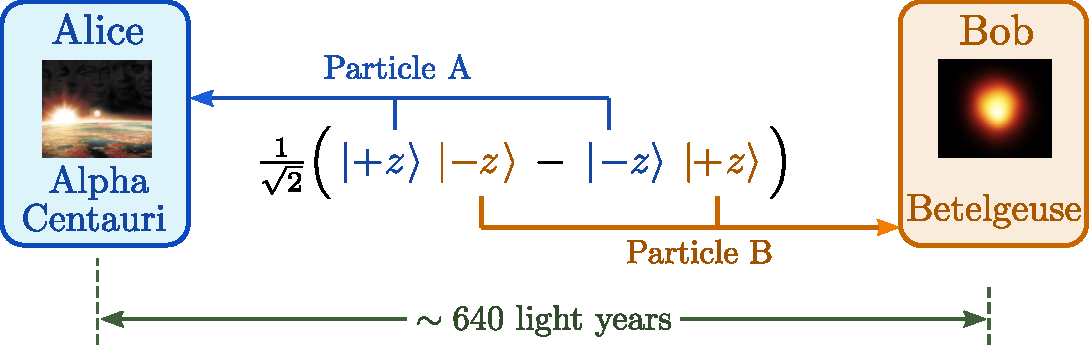
\includegraphics[width=0.6\textwidth]{epr}
\end{figure}

\noindent
In principle, this can be done carefully enough to avoid disturbing
the two-particle state.

At a pre-scheduled time, Alice measures $S_z$ on $A$.  As we saw
\hyperref[box:eproutcomes]{in the previous section}, her measurement
yields two equally probable outcomes.  If the result is $+\hbar/2$,
the combined state collapses to $|\!\uparrow\rangle
|\!\downarrow\rangle$; if the result is $-\hbar/2$, the combined state
collapses to $|\!\downarrow\rangle|\!\uparrow\rangle$.  Immediately
after Alice's scheduled measurement, Bob measures $\hat{S}_z$ on $B$.
He obtains, with 100\% probability, the result opposite to Alice's.

Notice that this thought experiment dispels some commonsensical but
mistaken explanations for state collapse.  For instance, it is
sometimes claimed that in order to measure a particle's position, we
must do something like shining light on it, which disturbs the
particle's state.  The EPR paradox shows that such stories do not
capture the full weirdness of quantum measurement.  We can collapse a
particle's quantum state without interacting directly with it, by
doing a measurement on another particle far away.

The postulates of quantum mechanics seem to indicate that the state
collapses instantaneously.  Alice and Bob are light years distant from
each other, so during the time interval between their measurements, no
classical signal could have passed between them, even at light speed.
Yet Alice's measurement evidently affects Bob's measurement.  Could
this be a violation of the theory of relativity?

Not so fast: to achieve an actual violation of relativity, Alice and
Bob must find a way to use the state collapse to perform superluminal
communication.  It is the combination of superluminal communication
with relativity that generates cause-and-effect inconsistencies, such
as the
\href{https://en.wikipedia.org/wiki/Temporal_paradox#Grandfather_paradox}{grandfather
  paradox}.  In the present setup, Alice and Bob individually see a
statistical distribution of measurement outcomes equivalent to a coin
flip (i.e., 50\% chance of getting $+\hbar/2$, and 50\% chance of
getting $-\hbar/2$).  Even if they repeat the experiment many times
with many independently-prepared singlet states, each of them only
receives a string of random bits, which carries no information.

Alice and Bob might try to get around this by varying their choice of
measurement.  For instance, instead of always measuring $S_z$, Alice
might choose to measure $S_x$.  This would cause the two-particle
state to collapse to something like
\begin{align*}
  |\!\rightarrow\rangle \otimes |\!\leftarrow\rangle &\qquad(\textrm{if Alice got $S_x = +\hbar/2$}) \\
  |\!\leftarrow\rangle \otimes |\!\rightarrow\rangle &\qquad(\textrm{if Alice got $S_x = -\hbar/2$}),
\end{align*}
instead of $|\!\uparrow\rangle |\!\downarrow\rangle$ and
$|\!\downarrow\rangle |\!\uparrow\rangle$.  If Bob could thereby
determine whether Alice had measured $S_x$ or $S_z$, this would be a
way to transmit one bit of information (e.g., $S_x$ means 1 and $S_z$
means 0) from Alice to Bob.  This would work even if the determination
is only statistical (e.g., if Bob can figure out that Alice picked
$S_x$ instead of $S_z$ with $50.1\%$ probability), since Alice and Bob
can simply repeat the experiment many times to reduce the uncertainty.

Upon closer inspection, it turns out that such schemes do \textit{not}
allow Alice and Bob to communicate.  The key point is that quantum
states themselves cannot be measured; only observables are measured.
By calculating the various measurement probabilities, we can prove the
following (see \hyperref[ex:singletproperties]{Exercise 1}):

\begin{itemize}
\item
  If Alice measures along axis $n$, and Bob then measures along axis
  $n'$, the overall probability for Bob to get either result (i.e.,
  $+\hbar/2$ or $-\hbar/2$) is 0.5, regardless of the choices of $n$
  and $n'$.

\item If $n = n'$, Bob always gets the opposite of Alice's result.
\end{itemize}

Since Bob always has equal probability to get either outcome, he is
unable to extract any information from the state collapse induced by
Alice.  This implies that the EPR thought experiment does not
contradict relativity.  Nonetheless, EPR argued that the situation is
unsatisfactory.  A central element of quantum theory---i.e., the
quantum state---is changing faster than the speed of light.  Even if
that change cannot be directly measured or used to transmit
information, this seems to violate the \textit{spirit} of relativity.

EPR suggested an alternative: maybe quantum mechanics is an
approximation of some deeper theory, whose details are currently
unknown.  Such a \textbf{hidden-variable theory} could give the
appearance of quantum state collapse, but without any
faster-than-light changes actually happening.

Suppose, contrary to quantum theory, that each particle has a definite
value of $S_z$, i.e., $S_z = +\hbar/2$ or $-\hbar/2$.  For simplicity,
let us denote these options as $+$ or $-$.  Let us hypothesize that
the two-particle quantum state $|\psi\rangle$ is actually a
statistical distribution of two kinds of ``\textbf{hidden-variable
  states}'': $\hvbox[+]{-}$ (i.e., $S_z = +\hbar/2$ for $A$ and $S_z =
-\hbar/2$ for $B$), or $\hvbox[-]{+}$ (vice versa).  When the state
$|\psi\rangle$ is prepared, one of these hidden-variable states is
randomly drawn from the distribution, but its contents are initially
hidden.

\begin{figure}[h]
  \centering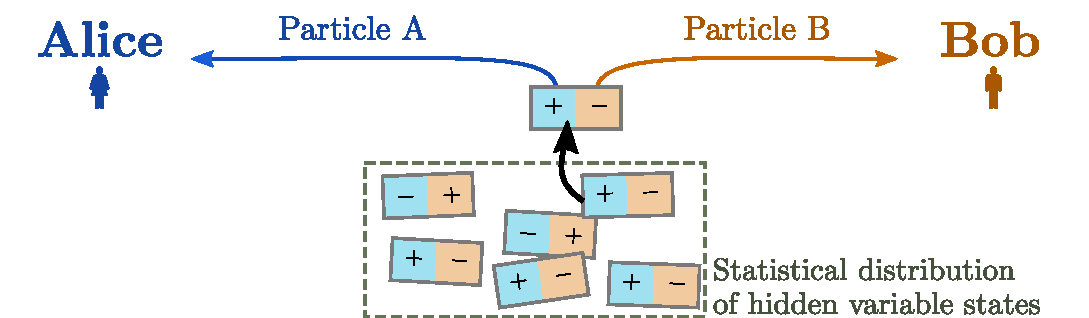
\includegraphics[width=0.7\textwidth]{hiddenvariables}
\end{figure}

When Alice measures $S_z$, the hidden variable is revealed.  If she
got $+$, that means the hidden-variable state must have been
$\hvbox[+]{-}$, whereas if she got $-z$, the hidden-variable state was
$\hvbox[-]{+}$.  When Bob subsequently measures $S_z$, his result will
be the opposite of Alice's.  These outcomes were predetermined when
the hidden-variable state was drawn, so there is no physical effect
traveling between Alice and Bob akin to the instantaneous state
collapse of quantum theory.

Clearly, there are many theoretical details missing.  The
hidden-variable theory would need to replicate all the successful
predictions made by quantum theory.  Trying to come up with a suitable
theory of this sort seems like a tall order, but with enough hard
work, might it be doable?

Well, no.

\section{Bell's theorem}
\label{sec:bell}

In 1964, Bell published a bombshell paper showing that the predictions
of quantum theory are inherently inconsistent with hidden-variable
theories [\ref{cite:bell}].  The amazing thing about this proof, which
is called \textbf{Bell's theorem}, is that it requires no knowledge
about the details of the hidden-variable theory, merely the fact that
it is deterministic and local.  Here, we present a simplified version
of Bell's theorem due to Mermin [\ref{cite:mermin}].

Yet again, we consider pairs of spin-1/2 particles, with particle $A$
sent to Alice and particle $B$ to Bob, with the two-particle state
\begin{equation}
  |\psi\rangle = \frac{1}{\sqrt{2}} \Big(|\!\uparrow\rangle|\!\downarrow\rangle \,-\, |\!\downarrow\rangle|\!\uparrow\rangle\Big).
  \label{bellsinglet}
\end{equation}
In each round of the thought experiment, Alice and Bob are each
allowed to measure their particle's spin along one of three possible
spin axes, whose observables are denoted by $S_1$, $S_2$, $S_3$ (we'll
specify the directions of these spin axes later).  Each
experimentalist chooses $S_1$, $S_2$, or $S_3$, \textit{randomly and
  with equal probabilities}.

Many rounds of the experiment are conducted.  Afterwards, we bring
together Alice's and Bob's experimental records, and examine their
axis choices and results.  For example:

\begin{figure}[h]
  \centering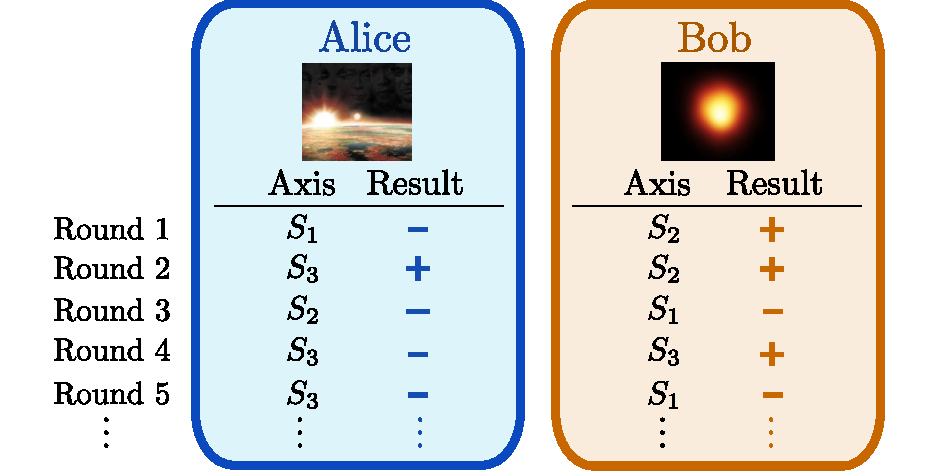
\includegraphics[width=0.6\textwidth]{bell}
\end{figure}

\noindent
If the results are consistent with quantum theory, whenever Alice and
Bob chose the same axis (by random chance), they must have obtained
opposite results.  For example, in the above records, they both chose
axis $S_3$ during Round 4; Alice got $-$, and Bob got $+$.

Can a hidden-variable theory reproduce such behavior?  In a
hidden-variable theory, each particle has a definite value for each
spin observable.  For example, $A$ might have $S_1 = +\hbar/2, \, S_2
= +\hbar/2, \, S_3 = -\hbar/2$, which we can denote more concisely as
`$++-$'.  For every spin axis, the two particles' hidden variables
must have opposite values.  Hence, there are $8$ possible
hidden-variable states, which we can denote like this:
\begin{align*}
  \begin{aligned}
    \hvbox[+++]{---} \;\;\;
    \hvbox[++-]{--+} \;\;\;
    \hvbox[+-+]{-+-} \;\;\;
    \hvbox[+--]{-++}\\
    \hvbox[-++]{+--} \;\;\;
    \hvbox[-+-]{+-+} \;\;\;
    \hvbox[--+]{++-} \;\;\;
    \hvbox[---]{+++}
  \end{aligned}
\end{align*}
For instance, $\hvbox[++-]{--+}$ indicates that $A$ has $S_1 = S_2 =
+\hbar/2$ and $S_3 = -\hbar/2$, while $B$ has $S_1 = S_2 = -\hbar/2$
and $S_3 = +\hbar/2$.  The hidden-variable theory postulates that the
two-particle state \eqref{bellsinglet} is actually some kind of
statistical distribution involving 8 hidden-variable states:
\begin{equation*}
  \Big\{ P\big(\hvbox[+++]{---}\,\big), \;P\big(\hvbox[++-]{--+}\,\big),
  \dots, P\big(\hvbox[---]{+++}\,\big) \Big\}.
\end{equation*}

Let us focus on the rounds in which Alice and Bob \textit{chose
  different spin axes}.  Within this subset, what is the probability
\textit{for their measurement results to have opposite signs}?  To
answer this question, we first consider these 6 hidden-variable
states:
\begin{align*}
  \begin{aligned}
    \hvbox[++-]{--+} \;\;\;
    \hvbox[+-+]{-+-} \;\;\;
    \hvbox[+--]{-++}\\
    \hvbox[-++]{+--} \;\;\;
    \hvbox[-+-]{+-+} \;\;\;
    \hvbox[--+]{++-}
  \end{aligned}
\end{align*}
These are the cases for which each particle's spin variables are not
all $+$ or all $-$.  Take the first case, $\hvbox[++-]{--+}$.  Under
our assumption that Alice and Bob chose different measurement axes,
there are two choices that give opposite signs for the measurement
results: $(S_1,S_2)$ or $(S_2,S_1)$.  Conversely, there are four
choices that give the same sign: $(S_1,S_3)$, $(S_2,S_3)$, $(S_3,S_1)$
and $(S_3, S_2)$.  Since the axis choices are totally random, the
probability of obtaining opposite signs for this hidden-variable state
is 1/3.  Going through the rest of the 6 hidden-variable states listed
above, we find that the probability to get opposite signs is likewise
1/3.  In the notation of conditional probabilities,
\begin{equation}
  P\big(\textrm{opp.} | \hvbox[++-]{--+}\,\big) =
  P\big(\textrm{opp.} | \hvbox[+-+]{-+-}\,\big) = \cdots = \frac{1}{3},
  \label{bell1}
\end{equation}
where ``opp.''~stands for opposite signs being obtained in the two
measurement results.

Now look at the remaining 2 hidden-variable states:
\begin{equation*}
    \hvbox[+++]{---} \;\;\;
    \hvbox[---]{+++}
\end{equation*}
For these, the conditional probabilities are
\begin{equation}
  P\big(\textrm{opp.} | \hvbox[+++]{---}\,\big) =
  P\big(\textrm{opp.} | \hvbox[---]{+++}\,\big) = 1.
  \label{bell2}
\end{equation}
By the law of conditional probabilities, the probability for the
``opposite signs'' outcome is
\begin{align}
  \begin{aligned}
    P\big(\textrm{opp.}\big) &= \;\;\;
    P\big(\textrm{opp.} | \hvbox[++-]{--+}\,\big)
    P\big(\hvbox[++-]{--+}\,\big) \\
    &\quad+ P\big(\textrm{opp.} | \hvbox[+-+]{-+-}\,\big)
    P\big(\hvbox[+-+]{-+-}\,\big) \\
    &\quad+ \quad \cdots \\
    &\quad+ P\big(\textrm{opp.} | \hvbox[---]{+++}\,\big)
    P\big(\hvbox[---]{+++}\,\big),
  \end{aligned}
\end{align}
where the sum runs over all 8 possibilities (hidden-variable states).
We can use Eqs.~\eqref{bell1} and \eqref{bell2} to insert the
conditional probabilities, resulting in
\begin{align}
  \begin{aligned}
    P\big(\textrm{opp.}\big) &=
    \frac{1}{3} \Big[\underbrace{P\big(\hvbox[++-]{--+}\,\big)
      + P\big(\hvbox[+-+]{-+-}\,\big)
      + \cdots + P\big(\hvbox[--+]{++-}\,\big)}_{\textrm{6 hidden-variable states
obeying Eq.~\eqref{bell1}}}\Big] \\
    &\quad + \underbrace{P\big(\hvbox[+++]{---}\,\big)
    + P\big(\hvbox[---]{+++}\,\big)}_{\textrm{2 hidden-variable states obeying \eqref{bell2}}}.
  \end{aligned}
\end{align}
It follows that
\begin{equation}
  P\big(\textrm{opp.}\big) \ge
  \frac{1}{3} \Big[\underbrace{P\big(\hvbox[++-]{--+}\,\big)
      + \cdots + P\big(\hvbox[---]{+++}\,\big)}_{\textrm{all 8 hidden-variable states}}
    \Big].
  \label{bellprob}
\end{equation}
The probabilities in the square brackets must sum to one.  Therefore,
\begin{equation}
  P\big(\textrm{opp.}\big) \ge \frac{1}{3}.
  \label{bellresult}
\end{equation}
This result, called \textbf{Bell's inequality}, can be summarized as
follows:

\begin{framed}
\noindent
\textit{In a hidden-variable theory, for the rounds where Alice and
  Bob choose different spin axes, their measurement results have
  opposite signs with probability $\ge 1/3$.}
\end{framed}

If we can find a situation where quantum theory predicts a violation
of Bell's inequality, that would prove quantum theory is inconsistent
with a broad class of hidden-variable theories.  It would not matter
how complicated the inner workings of the hidden-variable theory are,
so long as it meets the modest assumptions presented above (e.g.,
there are local deterministic hidden variables for each measurement,
the hidden-variable states are associated with probabilities summing
to one, etc.).

Thus, we seek a set of spin operators $\{S_1, S_2, S_3\}$ such that
quantum theory violates Bell's inequality.  One way to accomplish this
is to align $S_1$ with the $z$ axis, and place $S_2$ and $S_3$ in the
$x$-$z$ plane at $120^\circ$ ($2\pi/3$ radians) from $S_1$, as shown
below:

\begin{figure}[h]
  \centering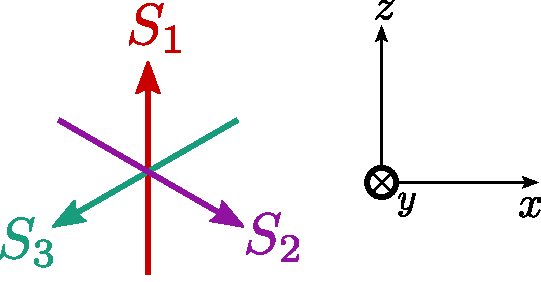
\includegraphics[width=0.25\textwidth]{bellaxes}
\end{figure}

\noindent
Using simple geometry, we can write $\{S_1, S_2, S_3\}$ in terms of
the Pauli matrices $\hat{\sigma}_1$ and $\hat{\sigma}_3$:
\begin{align}
  \begin{aligned}\hat{S}_1 &= \frac{\hbar}{2} \, \hat{\sigma}_3
    \\ \hat{S}_2 &= \frac{\hbar}{2} \, \left[\cos(2\pi/3) \hat{\sigma}_3 + \sin(2\pi/3)\hat{\sigma}_1\right]  \\   \hat{S}_3 &= \frac{\hbar}{2} \, \left[\cos(2\pi/3) \hat{\sigma}_3 - \sin(2\pi/3)\hat{\sigma}_1\right].\end{aligned}
\end{align}

For this choice of spin axes, suppose Alice chooses $S_1$ (i.e.,
$S_z$), and measures the result $+\hbar/2$.  Then the two-particle
state collapses to $|\!\uparrow\rangle |\!\downarrow\rangle$.  Bob is
assumed to choose a different spin axis.  If he chooses to measure
$S_2$, the expectation value for his measurement is
\begin{align}
  \langle\,\downarrow | \hat{S}_2 \,|\!\downarrow\,\rangle
  &= \frac{\hbar}{2} \,
  \Big[\cos(2\pi/3) \, \langle\,\downarrow|\sigma_3| \downarrow\,\rangle
    + \sin(2\pi/3)\, \langle\,\downarrow|\sigma_1|\downarrow\,\rangle\Big]\\
  &= \frac{\hbar}{2} \cdot \frac{1}{2}.
  \label{bellP}
\end{align}
We can also write this expectation value in terms of the probabilities
for Bob to measure $+\hbar/2$ and $-\hbar/2$, denoted by $P_B(+)$ and
$P_B(-)$ respectively:
\begin{align}
  \langle\,\downarrow | \hat{S}_2 \,|\!\downarrow\,\rangle
  &= \left[+\frac{\hbar}{2} P_B(+) - \frac{\hbar}{2} P_B(-)\right] \\
  &= \frac{\hbar}{2} \Big[P_B(+) - P_B(-)\Big].
  \label{bellP2}
\end{align}
Eqs.~\eqref{bellP} and Eq.~\eqref{bellP2} together imply that
\begin{equation}
  P_B(+) - P_B(-) = \frac{1}{2}.
\end{equation}
Moreover, by probability conservation,
\begin{equation}
  P_B(+) + P_B(-) = 1.
\end{equation}
Hence, the probability for Bob to obtain a negative value (the
opposite of Alice's result) is
\begin{equation}
  P_B(-) = \frac{1}{4}.
  \label{Bobresult}
\end{equation}
In a similar fashion, we can work through all the other possible
scenarios involving different choices of spin axes by Alice and Bob.
All yield the same result as Eq.~\eqref{Bobresult}: i.e., assuming
Alice and Bob chose different measurement axis, the probability for
them to obtain opposite results is $1/4$.  Bell's inequality is
violated!

Last of all, we must consult Nature.  Is it possible to experimentally
observe a violation of Bell's inequality?  In the decades following
Bell's paper, many experiments were performed to answer this question.
These experiments are all substantially more complicated than the
above toy model, and are subject to various real-world imperfections.
But in the end, the experimental consensus is a clear \textit{yes}:
Nature agrees with quantum mechanics, not the hidden-variable
theories!  The experimental evidence is reviewed in a paper by Aspect
[\ref{cite:aspect}].

\section{Quantum cryptography}

One of the most remarkable consequences of Bell's thought experiment
is that it provides a way to perform cryptography that is more secure,
in certain respects, than conventional cryptography.  The possibility
of \textbf{quantum cryptography} is poised to be one of the most
important technological applications of quantum entanglement.  Here,
we describe one of the earliest quantum cryptography schemes, devised
by Ekert in 1991 [\ref{cite:ekert}].

Ekert's scheme allows two participants, Alice and Bob, to share with
each other a string of random binary digits (0 or 1), called a
``key''.  The objective is to make this sharing secure, in the sense
that no one else can eavesdrop and learn the key.  After Alice and Bob
have established the key, they can use it alongside various
non-quantum methods to encrypt messages between each other (e.g., by using the key as a
\href{https://en.wikipedia.org/wiki/One-time_pad}{one-time pad}).

The scheme closely follows the Bell thought experiment from Section
\ref{sec:bell}.  Alice and Bob take part in multiple rounds of
measurements; during each round, a pair of spin-$1/2$ particles is
prepared in the singlet state \eqref{bellsinglet}, with particle $A$
going to Alice and $B$ going to Bob.  Each participant randomly
chooses an axis ($S_1$, $S_2$, or $S_3$), performs the corresponding
spin measurement, and secretly records down the result.

Alice and Bob then tell each other what axes they chose during the
measurement rounds.  These announcements are assumed to take place
over a communication channel that isn't necessarily secure, in the
sense that it might be eavesdropped upon; however, it is assumed that
the communications cannot be jammed or altered by any third party.
From this information, Alice and Bob identify the rounds in which they
picked the same axis (about 1/3 of the rounds), during which they must
have obtained exactly opposite measurement results.  These measurement
results are thus a string of random binary digits known to both Alice
and Bob, and no one else.

How might a third party, Eve, attempt to eavesdrop?  Suppose Eve was
able to intercept some or all of the $B$ particles intended for Bob.
She can try to extract some information from them (which, according to
quantum theory, means doing measurements on them), and then sending
some replacement particles to Bob (hoping he does not notice).
However, such measurements would break the entanglement between the
particles received by Alice and Bob.  The situation turns into a kind
of hidden-variable theory, where the hidden variables represent the
information extracted by Eve.

To check for Eve's tampering, Alice and Bob can publicly announce
their measurement results for the rounds in which their axes were
different.  (Remember, these rounds are not needed for the secret
key.)  Each of them can then check for a violation of Bell's
inequality, which would guarantee no eavesdropping has taken place.
For details, refer to Ref.~[\ref{cite:ekert}].

Alternatively, Eve might duplicate or ``clone'' the quantum state of
$B$ before it goes to Bob.  Then she can wait for Bob to announce his
choice of measurement axis for that round, perform that measurement on
her cloned particle, and reproduce Bob's result.  Though plausible at
first glance, this turns out to be incompatible with the laws of
quantum mechanics.

The so-called \textbf{no-cloning theorem} can be proven as follows.
Eve desires to clone an arbitrary state of a spin-half particle $B$
onto another spin-half particle $C$.  The two-particle Hilbert space
is $\mathscr{H}\otimes\mathscr{H}$.  With particle $C$ initially
prepared in some state $|0\rangle$, Eve must devise a unitary
operation $\hat{U}$, representing the cloning process, such that
\begin{equation}
  \hat{U} |\psi\rangle | 0\rangle = e^{i\phi} |\psi\rangle |\psi\rangle
  \label{clone}
\end{equation}
for all $|\psi\rangle \in \mathscr{H}$.  The phase factor $\phi$ can
depend on $|\psi\rangle$.

Now replace $|\psi\rangle$ in the above equation with two arbitrary
states denoted by $|\psi_1\rangle$ and $|\psi_2\rangle$, and take
their inner product.  According to Eq.~\eqref{clone},
\begin{align}
  \Big(\langle \psi_1 | \langle 0 | \hat{U}^\dagger \Big)
  \Big(\hat{U} | \psi_2 \rangle |0\rangle \Big)
  &=  \Big(\langle \psi_1| \langle \psi_1| e^{-i\phi_1} \Big) \Big( e^{i\phi_2} |\psi_2\rangle|\psi_2\rangle\Big) \\
  &= e^{-i(\phi_1-\phi_2)} \Big( \langle\psi_1 | \psi_2\rangle \Big)^2. \label{clone1}
\end{align}
Here, $\phi_1$ and $\phi_2$ are the phase factors from
Eq.~\eqref{clone} for the two chosen states.  On the other hand, since
$\hat{U}$ is unitary,
\begin{align}
  \langle \psi_1 | \langle 0 | \hat{U}^\dagger \hat{U} | \psi_2 \rangle |0\rangle
  &= \Big(\langle \psi_1 | \langle 0| \Big) \Big(| \psi_2 \rangle |0\rangle\Big)
  \\ &= \langle\psi_1 | \psi_2\rangle. \label{clone2}
\end{align}
Comparing the magnitudes of \eqref{clone1} and \eqref{clone2},
\begin{equation}
  \big|\langle \psi_1 | \psi_2\rangle \big|^2
  = \big| \langle\psi_1 | \psi_2\rangle \big|
  \;\;\Rightarrow \;\;
  \big|\langle\psi_1 | \psi_2\rangle\big| = 0 \;\mathrm{or}\; 1.
\end{equation}
But aside from the trivial case of a one-dimensional Hilbert space,
this cannot be true for arbitrary $|\psi_1\rangle$ and
$|\psi_2\rangle$.  For instance, for a two-dimensional space spanned
by an orthonormal basis $\{|0\rangle, |1\rangle\}$, we can pick
\begin{equation}
  |\psi_1\rangle = |0\rangle, \;
  |\psi_2\rangle = \frac{1}{\sqrt{2}}\big(|0\rangle +
  |1\rangle\big)
  \;\;\Rightarrow\;\;
  \big|\langle\psi_1|\psi_2\rangle\big| = \frac{1}{\sqrt{2}}.
\end{equation}

\section{Density operators}

We now introduce \textbf{density operators}, which help streamline
calculations involving systems of multiple particles (or, more
generally, multiple subsystems).

As a warm-up, consider a quantum system in a state $|\psi\rangle \in
\mathscr{H}$.  We can define the Hermitian operator
\begin{equation}
  \hat{\rho} = |\psi\rangle\, \langle\psi|.
  \label{rho_pure}
\end{equation}
This is just the projector for $|\psi\rangle$, but in this context we
call it a ``density operator''.  It is also commonly called a
\textbf{density matrix}.

In Section~\ref{sec:partialmeasurements}, we had gone through the
rules for calculating the probabilities for measurements done on
$|\psi\rangle$.  Using $\hat{\rho}$, these rules can be re-stated as
follows:

\begin{enumerate}
\item If we measure an observable $\hat{Q}$, whose eigenvalues are
  $\{q\}$ and eigenstates are $\{|q\rangle\}$, the probability of
  obtaining $q$ is
  \begin{equation}
    P(q) = \big|\langle q | \psi\rangle\big|^2 =
    \langle \mu |\, \hat{\rho}\, | \mu \rangle.
    \label{Pi_rho}
  \end{equation}

\item The expectation value of the observable is
  \begin{equation}
    \langle Q\rangle
    = \sum_q q P(q)
    = \sum_q \langle q | \hat{Q}\, \hat{\rho}| q \rangle
    = \mathrm{Tr}\big[\,\hat{Q} \, \hat{\rho}\,\big].
    \label{Qexpt}
  \end{equation}
  Here, $\mathrm{Tr}[\cdots]$ denotes the trace, which is the sum of
  the diagonal elements of the matrix representation of the operator.
  Its value is basis independent.
\end{enumerate}

Let us move on to partial measurements.  Consider, once again, two
subsystems $A$ and $B$, with Hilbert spaces $\mathscr{H}_A$ and
$\mathscr{H}_B$.  Suppose we are specifically interested in partial
measurements performed on $A$.  As detailed in
Section~\ref{sec:partialmeasurements} the probabilities of these
partial measurement outcomes can be calculated from the state of the
combined system,
\begin{equation*}
  |\psi\rangle \in \mathscr{H}_A\otimes \mathscr{H}_B.
\end{equation*}
However, $|\psi\rangle$ also contains information about $B$, which we
are not interested in.  Is there a more economical way to encode just
the properties of the $A$ subsystem?

To do this, we define the density operator for $A$, sometimes called
the \textbf{reduced density operator}, as follows:
\begin{equation}
  \hat{\rho}_A = \mathrm{Tr}_B \,\big[\,\hat{\rho}\,\big].
  \label{rhoa_def}
\end{equation}
Here, $\hat{\rho}$ is the density matrix for the combined system, as
defined in Eq.~\eqref{rho_pure}.  $\mathrm{Tr}_B[\cdots]$ denotes a
\textbf{partial trace}, which means tracing out the $B$ part of the
Hilbert space.  To be precise, given a basis $\{|\beta\rangle\}$ for
$\mathscr{H}_B$, the partial trace is
\begin{equation}
  \hat{\rho}_A =
    \sum_\beta
    \Big( \hat{I}\otimes \langle \beta| \Big)
    \; |\psi\rangle \langle \psi | \;
    \Big( \hat{I}\otimes | \beta\rangle \Big).
    \label{rhoa_explicit}
\end{equation}
In the $A$ part of the Hilbert space, we do nothing (i.e., apply
identity operators), while in the $B$ part we perform a trace.
Whereas the standard trace turns an operator to a scalar, this partial
trace turns an operator acting on $\mathscr{H}_A \otimes
\mathscr{H}_B$ into an operator acting on just $\mathscr{H}_A$.  Like
the standard trace, the partial trace turns out to be basis
independent---i.e., even if we use a different basis in
Eq.~\eqref{rhoa_explicit}, we end up with the same operator.

Now, suppose we measure an observable $\hat{Q}_A$ on subsystem $A$,
which has eigenstates $\{|\alpha\rangle\}$ and eigenvalues
$\{\alpha\}$.  According to the rules for partial measurements
(Section~\ref{sec:partialmeasurements}), the probability of obtaining
$\alpha$ is
\begin{align}
  P(\alpha)
    &=
    \langle \psi | \,
    \Big( |\alpha\rangle \langle \alpha| \otimes \hat{I}_B\Big) |\psi\rangle \\
    &=
    \langle \psi | \,
    \left[ |\alpha\rangle \langle \alpha| \otimes
      \left(\sum_\beta | \beta\rangle \langle \beta|\right) \right]
    |\psi\rangle \\
    &=
    \sum_\beta
    \Big( \langle \alpha| \langle \beta| \Big)
    \, |\psi\rangle \langle \psi | \,
    \Big( |\alpha\rangle | \beta\rangle \Big) \\
    &= \langle \alpha | \hat{\rho}_A | \alpha \rangle.
    \label{rho_prob}
\end{align}
This result is clearly analogous to Eq.~\eqref{Pi_rho}.  Hence, we can
use $\hat{\rho}_A$ to directly calculate the probabilities for any
measurement on $A$.  As a corollary,
\begin{equation}
  \langle Q_A \rangle = \sum_\alpha \alpha
  \langle \alpha | \hat{\rho}_A | \alpha \rangle
  = \mathrm{Tr}\Big[\hat{Q}_A \, \hat{\rho}_A \Big],
  \label{rho_expect}
\end{equation}
which is analogous to Eq.~\eqref{Qexpt}.
    
To better understand these results, let us expand the state of the
combined system as
\begin{equation}
  |\psi\rangle = \sum_{\alpha\beta} \psi_{\alpha\beta} |\alpha\rangle |\beta\rangle,
\end{equation}
where $\sum_{\alpha\beta} |\psi_{\alpha\beta}|^2 = 1$.  Then
\begin{equation}
  \hat{\rho} = \sum_{\alpha\alpha'\beta\beta'} \psi_{\alpha\beta}
  \psi_{\alpha'\beta'}^* \; |\alpha\rangle |\beta\rangle \,
  \langle\alpha'|\langle \beta'|,
\end{equation}
and the reduced density operator is
\begin{align}
  \begin{aligned}
    \hat{\rho}_A &= \sum_{\alpha\alpha'\beta} \psi_{\alpha\beta}\psi_{\alpha'\beta}^* |\alpha\rangle
    \langle\alpha'| \\
    &= \sum_\beta \left(\sum_\alpha \psi_{\alpha\beta} |\alpha\rangle\right)
    \left(\sum_{\alpha'} \psi_{\alpha'\beta}^*\langle\alpha'|\right) \\
    &= \sum_\beta |\varphi_\beta\rangle \langle \varphi_\beta|,
    \;\;\;\mathrm{where}\;\;\;
    |\varphi_\beta\rangle = \sum_\alpha \psi_{\alpha\beta} |\alpha\rangle.
  \end{aligned}
  \label{rhoa_tmp}
\end{align}
But $|\varphi_\beta\rangle$ is not necessarily normalized to unity:
\begin{equation}
  \langle \varphi_\beta | \varphi_\beta\rangle =
  \sum_{\alpha}|\psi_{\alpha\beta}|^2 \le 1.
\end{equation}
Let us therefore define the re-normalized states
\begin{equation}
  |\Psi_\beta\rangle = \frac{1}{\sqrt{P_\beta}} |\varphi_\beta\rangle,
  \;\;\;\mathrm{where} \;\; P_\beta = \sum_{\alpha}|\psi_{\alpha\beta}|^2.
\end{equation}
Note that each $P_\beta$ is a non-negative real number in the range
$[0,1]$.  Eq.~\eqref{rhoa_tmp} now becomes
\begin{equation}
  \hat{\rho}_A = \sum_\beta P_\beta\, |\Psi_\beta\rangle
  \langle \Psi_\beta|,
  \;\;\;\mathrm{where}\;\;
  \begin{cases}
    \;\;\textrm{each $P_\beta$ is a real number in $[0,1]$, and} \\
    \;\;\textrm{each}\; |\Psi_\beta\rangle \in \mathscr{H}_A,
    \;\;\mathrm{with}
    \;\;\langle\Psi_\beta|\Psi_\beta\rangle = 1.
  \end{cases}
  \label{rhoform}
\end{equation}
This has the form of a sum of density operators for a set of quantum
states $\{|\Psi_\beta\rangle\}$, weighted by a set of classical
probabilities $\{P_\beta\}$.  This called an \textbf{ensemble} of
states.  Note that the states in the ensemble need not be orthogonal
to each other.

Although we have derived Eq.~\eqref{rhoform} from $|\psi\rangle$, the
state of the combined system, we cannot work backwards from
$\hat{\rho}_A$ to figure out $|\psi\rangle$ (specifically, the
coefficients $\psi_{\alpha\beta}$).  In other words, $\hat{\rho}_A$
provides all the necessary information regarding measurements on $A$,
discarding extraneous information about subsystem $B$ and how it is
entangled with $A$.  This means that we don't have to keep thinking of
$\hat{\rho}_A$ as a reduced density operator derived from some larger
state; we can simply present it as ``the density operator for $A$''.

From this point of view, a density operator of the form
$|\psi\rangle\langle\psi|$, which we started with back in
Eq.~\eqref{rho_pure}, is the special case of an ensemble of one
quantum state $|\psi\rangle$ with probability $P = 1$.  We call such
an ensemble a \textbf{pure state}.  If an ensemble is not a pure
state, we call it a \textbf{mixed state}, and this implies that the
system is entangled with something else.

Using Eq.~\eqref{rhoform}, we can show that the density matrix
$\hat{\rho}_A$ (be it for a pure state or a mixed state) has the
following properties:
\begin{enumerate}
\item $\hat{\rho}_A$ is Hermitian.

\item $\langle\varphi|\hat{\rho}_A|\varphi\rangle \ge 0$ for any
  $|\varphi\rangle \in \mathscr{H}_A$ (i.e., the operator is positive
  semidefinite).

\item For any observable $\hat{Q}_A$ acting on $\mathscr{H}_A$,
  \begin{align}
    \begin{aligned}
      \langle Q_A \rangle
      %% &\equiv \sum_\beta P_\beta
      %% \langle \Psi_\beta|\hat{Q}_A|\Psi_\beta\rangle \\
      %% &= \sum_{\alpha\beta} P_\beta\,
      %% \langle \Psi_\beta|\alpha\rangle \,
      %% \langle\alpha|\hat{Q}_A|\Psi_\beta\rangle
      %% \;\;\;\big(\textrm{using some basis} \;\{|\alpha\rangle\}\big) \\
      %% &= \sum_\alpha
      %% \langle\alpha|\hat{Q}_A \left(\sum_\beta |\Psi_\beta\rangle
      %% \langle \Psi_\beta|\right) |\alpha\rangle \\
      &= \mathrm{Tr}\left[\,\hat{Q}_A \,\hat{\rho}_A\,\right].
    \end{aligned}
    \label{prop3}
  \end{align}
  This also gives the probability for any measurement outcome: if
  $|\alpha\rangle$ is the eigenstate associated with the outcome, the
  outcome probability is $\langle\alpha|\hat\rho_A|\alpha\rangle$,
  consistent with Eq.~\eqref{rho_prob}.  To see this, take $\hat{Q}_A
  = |\alpha\rangle \langle \alpha|$.
  
\item The eigenvalues of $\hat{\rho}_A$, denoted by $\{p_1, p_2,
  \dots, p_{d_A}\}$, form a set of probabilities.  In other words,
  they satisfy
  \begin{equation}
    p_j \in \mathbb{R} \;\;\;\mathrm{and}\;\; 0 \le p_j \le 1 \;\;
    \mathrm{for}\;\; j = 1,\dots,d_A,
    \quad\mathrm{with}\;\; \sum_{j=1}^{d_A} p_j = 1.
    \label{trrho_reduced}    
  \end{equation}
  From this, it directly follows that
  \begin{equation}
    \mathrm{Tr}[\hat\rho_A] = 1.
  \end{equation}
  Property 4 follows from Property 3.  First, take $\hat{Q}_A =
  |j\rangle\langle j|$, where $|j\rangle$ is any eigenvector of
  $\hat\rho_A$ with eigenvalue $p_j$, and use Property 3 to prove that
  $0 \le p_j \le 1$.  Then take $\hat{Q} = \hat{I}_A$ and use Property
  3 to prove that the eigenvalues sum to 1.
\end{enumerate}

In some circumstances, we can assume that a system is in a given mixed
state, without deriving its density matrix via a partial trace.  For
example, if a system has energy eigenbasis $\{|\psi_n\rangle\}$ and
energies $\{E_n\}$, and is in thermal equilibrium with an external
heat bath of temperature $T$, its density operator can be assumed to
be
\begin{equation}
  \hat{\rho}_A = \sum_{n} \frac{\exp(-E_n/k_BT)}{Z} \, |E_n\rangle\langle E_n|,
\end{equation}
where $Z = \sum_n \exp(-E_n/k_BT)$.  This is justified by the
postulates of statistical mechanics, rather than any actual derivation
based on tracing out the heat bath's quantum degrees of freedom, which
would be hopelessly complicated.  So long as the weights in the sum
are classical probabilities (i.e., non-negative real numbers adding up
to 1), the density matrix $\hat{\rho}_A$ will satisfy the general
properties 1--4 described above.

\section{Entanglement entropy}
\label{sec:entropy}

Previously, we said that a multi-particle system is entangled if the
individual particles lack definite quantum states.  It would be nice
to make this statement more precise, and in fact physicists have come
up with several different quantitive measures of entanglement.  In
this section, we will describe the most common measure,
\textbf{entanglement entropy}, which is closely related to the
``entropy'' concept from thermodynamics, statistical mechanics, and
information theory.

We have seen from the previous section that if a subsystem $A$ is
(possibly) entangled with some other subsystem $B$, the information
required to calculate all partial measurement outcomes on $A$ is given
by a reduced density operator $\hat{\rho}_A$.  We can use this to
define a quantity called the \textbf{entanglement entropy} of $A$:
\begin{equation}
  S_{A} = - k_b \, \mathrm{Tr}_A \Big\{ \hat{\rho}_A\, \ln\!\big[\hat{\rho}_A\big]\Big\}.
  \label{entropy}
\end{equation}
In this formula, $\ln[\cdots]$ denotes the logarithm of an operator,
which is the inverse of the exponential: $\ln(\hat{P}) = \hat{Q}
\Rightarrow \exp(\hat{Q}) = \hat{P}$.  The prefactor $k_b$ is
Boltzmann's constant, and ensures that $S_A$ has the same units as
thermodynamic entropy.

In classical statistical mechanics, entropy is a quantitative measure
of uncertainty (i.e, lack of information) about a system's underlying
microscopic state, or ``microstate''.  Suppose a system has $W$
possible microstates occurring with probabilities $\{p_1, p_2, \dots,
p_W\}$.  Then the classical entropy is defined as
\begin{equation}
  S_{\mathrm{cl.}} = - k_b \sum_{i=1}^W p_i \ln(p_i).
  \label{Scl}
\end{equation}
It can be shown (see Appendix C) that for \textit{any} probability
distribution,
\begin{equation}
  0 \le S_{\mathrm{cl.}} \le k_b\ln W.
\end{equation}
The lower bound, $S_{\mathrm{cl.}} = 0$, occurs if and only if $p_i =
\delta_{ik}$ for a specific $k$, which can be interpreted as a
situation of ``complete certainty'' about the microstate.  The upper
bound, $S_{\mathrm{cl.}} = k_b\ln W$, occurs if and only if all
microstates are equally probable (i.e., $p_i = 1/W$), which
corresponds to ``complete uncertainty'' about the system's microstate.

The entanglement entropy \eqref{entropy} similarly aims to quantify
the uncertainty arising from a quantum system's lack of a definite
quantum state, due to it being possibly entangled with another system.
In formulating this concept, we need to be careful about how classical
notions of probability apply to quantum systems.  We have seen that
when performing a measurement on $A$ whose possible outcomes are
$\{q\}$, the probability of each outcome is $P(q) = \langle q |
\hat{\rho}_A|q\rangle$.  However, it is problematic to directly
substitute these probabilities $\{P(q)\}$ into the classical entropy
formula \eqref{Scl}, since they are basis-dependent.
Eq.~\eqref{entropy} bypasses this problem by using the trace, which is
basis-independent.

In one specific basis, the eigenbasis for $\hat{\rho}_A$, the
entanglement entropy does match the classical entropy formula.  Let
$\{|\mu\rangle\}$ be the eigenstates of $\hat{\rho}_A$; as shown in
Eq.~\eqref{trrho_reduced}, the corresponding eigenvalues $\{p_\mu\}$
form a set of probabilities.  Then
\begin{align}
  \begin{aligned}
    S_A &= -k_b \sum_\mu \langle \mu | \hat{\rho}_A \ln(\hat{\rho}_A) | \mu\rangle  \\
    &= - k_b \sum_\mu p_\mu \ln(p_\mu).
    \label{SAmu}
  \end{aligned}
\end{align}
From this, we can see that the entanglement entropy obeys the
following bounds, similar to the classical entropy formula:
\begin{equation}
  0 \le S_A \le k_b\ln(d_A), \quad
  \mathrm{where}\; d_A = \mathrm{dim}\left[\mathscr{H}_A\right].
  \label{Sabounds}
\end{equation}
The lower bound, $S_A = 0$, holds if and only if one of the $p_\mu$'s
in Eq.~\eqref{SAmu} is 1, and all the others are zero, meaning $A$ is
in a pure state.  Conversely, $S_{A} \ne 0$ when $\hat{\rho}_A$
describes a mixed state---i.e., $A$ is entangled with some other
quantum system.

A system is said to be \textbf{maximally entangled} if it saturates
the upper bound of \eqref{Sabounds}.  This occurs if and only if the
eigenvalues of the density operator are all equal to $1/d_A$.

\begin{framed}
\noindent
\textit{Example}---Consider the singlet state
\begin{align}
  |\psi\rangle = \frac{1}{\sqrt{2}} \Big(|\!\uparrow\rangle|\!\downarrow\rangle \,-\, |\!\downarrow\rangle|\!\uparrow\rangle\Big).
\end{align}
The corresponding density operator is
\begin{equation}
  \hat{\rho}(\psi) = \frac{1}{2} \Big(|\!\uparrow\rangle|\!\downarrow\rangle \,-\, |\!\downarrow\rangle|\!\uparrow\rangle\Big) \Big(\langle\uparrow\!|\langle\downarrow\!| \,-\, \langle\downarrow\!|\langle\uparrow\!|\Big).
\end{equation}
Tracing over system $B$ (the second slot) yields the reduced density operator
\begin{equation}
  \hat{\rho}_A(\psi) = \frac{1}{2} \Big(|\!\uparrow\rangle \langle\uparrow\!| \,+\, |\!\downarrow\rangle \langle\downarrow\!|\Big).
\end{equation}
This can be expressed as a matrix in the
$\{|\!\uparrow\rangle,|\!\downarrow\rangle\}$ basis:
\begin{equation}
  \hat{\rho}_A(\psi) = \begin{pmatrix}\frac{1}{2} & 0 \\ 0 & \frac{1}{2}\end{pmatrix}.
\end{equation}
Now we can use $\hat{\rho}_A$ to compute the entanglement entropy:
\begin{equation}
  S_A = -k_b\mathrm{Tr}\left\{\hat{\rho}_A\ln(\rho_A)\right\} = -k_b\mathrm{Tr}\begin{pmatrix}\frac{1}{2}\ln\left(\frac{1}{2}\right) & 0 \\ 0 & \frac{1}{2}\ln\left(\frac{1}{2}\right)\end{pmatrix} = k_b\ln(2).
\end{equation}
Hence, $A$ and $B$ are maximally entangled.
\end{framed}

\section{The Many Worlds Interpretation}

We conclude this chapter with a set of interesting but controversial
ideas related to the entanglement phenomenon: the \textbf{Many Worlds
  Interpretation} of quantum mechanics [\ref{cite:everett}].

So far, when describing the phenomenon of state collapse, we have
relied on the measurement postulate (see
Section~\ref{sec:partialmeasurements}), which is part of the
\textbf{Copenhagen Interpretation} of quantum mechanics.  This is how
quantum mechanics is typically taught, and also how physicists usually
think about measurement when doing practical calculations.

However, the measurement postulate has two bad features:

\begin{enumerate}
\item It stands apart from the other postulates of quantum mechanics
  as the only place where randomness (or ``indeterminism'') creeps
  into quantum theory.  The other postulates do not refer to
  probabilities.  In particular, the Schr\"odinger equation
\begin{equation}
  i\hbar\frac{\partial}{\partial t}|\psi(t)\rangle = \hat{H}(t) |\psi(t)\rangle
\end{equation}
is completely deterministic.  If you know $\hat{H}(t)$ and the initial
state $|\psi(t_0)\rangle$ at time $t_0$, you can in principle
calculate $|\psi(t)\rangle$ for all $t$.  This time evolution
describes a smooth, deterministic rotation of the state vector.  A
measurement process is completely different: during state collapse,
the state vector jumps instantaneously to a random value.  It seems
strange for quantum theory to contain two completely different ways
for a state to change.

\item The measurement postulate is silent on what constitutes a
  measurement.  Does measurement require a conscious observer?  Surely
  not: as Einstein once exasperatedly asked, are we to believe that
  the Moon exists only when we look at it?  But if a given device
  interacts with a particle, what determines whether it acts via the
  Schr\"odinger equation, or performs a measurement?
\end{enumerate}

The Many Worlds Interpretation of quantum mechanics seeks to resolve
these problems by positing that the measurement postulate is
\textit{not} a fundamental postulate of quantum mechanics.  It says
that the key features of quantum measurement---e.g., the randomness of
outcomes, and the quantum state collapsing after a measurement---are
emergent properties of large and complex quantum systems obeying the
Schr\"odinger equation.  They can be derived, rather than posited, by
adopting quantum descriptions for both the system being measured
\textit{and} the system doing the measurement.

We can use a toy model to illustrate this idea [\ref{cite:albrecht}].
Suppose we have (i) a spin-$1/2$ particle, whose Hilbert space is
$\mathscr{H}_S$, and (ii) an apparatus that measures $S_z$ on that
particle, whose Hilbert space is $\mathscr{H}_A$.  The apparatus has a
vast number of degrees of freedom, for it comprises a macroscopic
device that performs the $S_z$ measurement (and, optionally, an
experimentalist who looks at the result, etc.).  Its Hilbert space
thus has a mind-bogglingly high dimension:
\begin{equation}
  d_A = \mathrm{dim}[\mathscr{H}_A] \gg 1.
\end{equation}
The Hilbert space for the combined system of spin and apparatus is
\begin{equation}
  \mathscr{H}_S \otimes \mathscr{H}_A.
\end{equation}

Let us suppose the combined system is prepared in an initial state
\begin{equation}
  |\psi(0)\rangle = \Big(a_1 |\!\uparrow\rangle + a_2 |\!\downarrow\rangle\Big) \otimes |\Psi\rangle,
  \label{psi0_albrecht}
\end{equation}
where $a_1$ and $a_2$ are the spin-up and spin-down quantum
amplitudes, and $|\Psi\rangle \in \mathscr{H}_A$ is some initial state
for the apparatus, which is initially not entangled with the spin.

We aim to show that the apparatus behaves as though is ``measuring''
the spin, simply by evolving the combined system using a Hamiltonian
of the form
\begin{equation}
  \hat{H} = \hat{S}_z \otimes \hat{V}.
  \label{V_albrecht}
\end{equation}
This will only involve unitary time evolution via the Schr\"odinger
equation, \textit{without} invoking the measurement postulate.  Also,
it turns out that we will not need to make any special choices for
$|\Psi\rangle$ in Eq.~\eqref{psi0_albrecht}, or $\hat{V}$ in
Eq.~\eqref{V_albrecht}, so we leave these unspecified for now.

The assumed Hamiltonian \eqref{V_albrecht} is time-independent, so the
state after some time $t$ is
\begin{equation}
  |\psi(t)\rangle = e^{-i\hat{H}t/\hbar}\, |\psi(0)\rangle.
  \label{mwi_psit}
\end{equation}
To find this, observe how the Hamiltonian \eqref{V_albrecht} acts on
each term of the initial state defined in Eq.~\eqref{psi0_albrecht}:
\begin{align}
  \hat{H} |\!\uparrow\rangle |\Psi\rangle
  &= + \frac{\hbar}{2}\;
  |\!\uparrow\rangle \otimes \left(\hat{V} |\Psi\rangle\right), \\
  \hat{H} |\!\downarrow\rangle |\Psi\rangle
  &= - \frac{\hbar}{2}\;
  |\!\downarrow\rangle \otimes \left( \hat{V} |\Psi\rangle\right).
\end{align}
Hence,
\begin{equation}
  e^{-i\hat{H}t/\hbar}\, 
  |\!\updownarrow\rangle |\Psi\rangle
  = |\!\updownarrow\rangle \otimes
  \left(e^{\mp i\hat{V}t/2} |\Psi\rangle\right).
\end{equation}
Applying this to Eq.~\eqref{mwi_psit} yields
\begin{equation}
  |\psi(t)\rangle =
  a_1 |\!\uparrow\rangle |\Psi_\uparrow(t)\rangle + a_2 |\!\downarrow\rangle  |\Psi_\downarrow(t)\rangle,
  \label{psit}
\end{equation}
where
\begin{equation}
  |\Psi_{\updownarrow} (t)\rangle = e^{\mp i\hat{V}t/2} |\Psi\rangle
  \;\;\in\, \mathscr{H}_A.
\end{equation}

Based on Eq.~\eqref{psit}, we can interpret $|\Psi_\uparrow(t)\rangle$
and $|\Psi_\downarrow(t)\rangle$ as apparatus states corresponding to
each possible measurement result.  For example,
$|\Psi_\uparrow(t)\rangle$ may represent a state in which the device
has printed a message saying ``$S_z = + \hbar/2$'' on its screen;
also, if the apparatus subsystem contains an experimentalist, that
person has read the message and observed that the result is spin-up.
For this interpretation to work, $|\Psi_\uparrow(t)\rangle$ and
$|\Psi_\downarrow(t)\rangle$ ought to be almost exactly orthogonal,
since they refer to utterly different states of $\mathscr{H}_A$.  This
turns out to be readily satisfied; we will show (and later verify
numerically) that if $d_A \gg 1$,
\begin{equation}
  \langle\Psi_\uparrow(t) | \Psi_\downarrow(t)\rangle \rightarrow 0
  \label{overlapzero}
\end{equation}
after the passage of a short time $t$.

In the Many Worlds Interpretation, the two terms in Eq.~\eqref{psit}
represent two disinct ``worlds''.  Within each world, it appears that
the spin has collapsed to a particular eigenstate, and the apparatus
has measured the corresponding value of $S_z$.  But from the point of
view of the combined state $|\psi(t)\rangle$, which contains both
worlds, the spin and apparatus are entangled.  The two worlds'
relative importance is quantified by the weights $|a_1|^2$ and
$|a_2|^2$, which are precisely the two measurement probabilities
specified by the initial state \eqref{psi0_albrecht}.

To back this up, let us perform an explicit numerical calculation.
Since we have little hope of formulating a realistic model for a
measurement apparatus, let us choose the apparatus state
$|\Psi\rangle$ in Eq.~\eqref{psi0_albrecht}, and the operator
$\hat{V}$ in Eq.~\eqref{V_albrecht}, in a generic way.  For
$|\Psi\rangle$, we pick a random complex vector in an arbitrary basis,
with each component having its real and imaginary parts drawn from the
normal distribution $N(0,1)$:
\begin{equation}
  |\Psi\rangle = \frac{1}{\sqrt{\mathcal{N}}}\, \begin{pmatrix}
    \Psi_1 \\ \vdots \\ \Psi_{d_A}
  \end{pmatrix}, \;\; \mathrm{where} \;\; \mathrm{Re}(\Psi_j), \mathrm{Im}(\Psi_j) \sim N(0,1).
\end{equation}
Here, the constant $\mathcal{N}$ is chosen so that $|\Psi\rangle$ is
normalized to unity.  Similarly, we let $\hat{V}$ be a random
Hermitian $d_A\times d_A$ matrix:
\begin{equation}
  \hat{V} = \frac{1}{2\sqrt{d_A}} \left(\hat{A} + \hat{A}^\dagger\right),
  \;\; \mathrm{where} \;\; \mathrm{Re}(A_{ij}), \mathrm{Im}(A_{ij}) \sim N(0,1).
  \label{gue}
\end{equation}
(The prefactor of $1/2\sqrt{d_A}$ is unimportant for our present
discussion; it simply ensures that the eigenvalues of $\hat{V}$ lie in
the range $[-2,2]$ rather than scaling with $d_A$, according to the
theory of random matrices [\ref{cite:edelman}].)  In this example, we
will choose $d_A = 100$.

Now we simply have to pick the inital state (say, $a_1 = 0.7$ and $a_2
= \sqrt{1-a_1^2}$), and solve the Schr\"odinger equation numerically
(for details, refer to Appendix D).  Then we can generate plots like
this:

\begin{figure}[h]
  \centering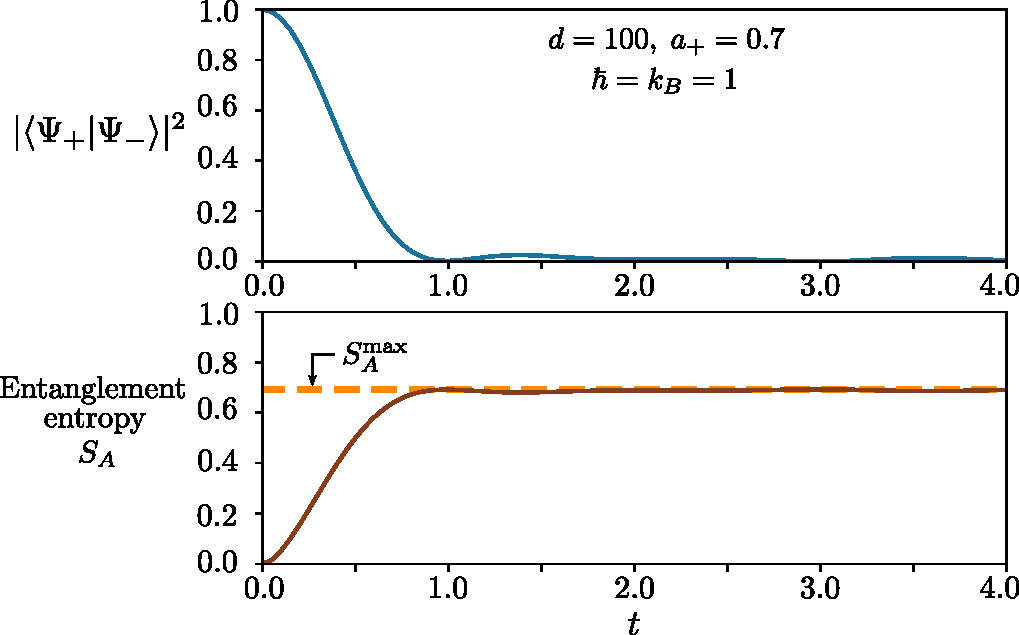
\includegraphics[width=0.7\textwidth]{decoherence}
\end{figure}

The upper plot shows $|\langle\Psi_\uparrow|\Psi_\downarrow\rangle|^2$
versus $t$.  This is equal to 1 at $t = 0$, but then drops rapidly to
around zero, and stays there, in agreement with
Eq.~\eqref{overlapzero}.

The lower plot shows the entanglement entropy of the spin and
apparatus (see Section~\ref{sec:entropy}).  At $t = 0$, this is zero,
consistent with the two subsystems being initially unentangled
[Eq.~\eqref{psi0_albrecht}].  Subsequently, $S_A$ increases up to
\begin{equation}
  S_A^{\mathrm{max}} = - k_b \Big( |a_1|^2 \ln|a_1|^2 + |a_2|^2\ln|a_2|^2 \Big) \approx 0.693 \,k_b.
\end{equation}
This corresponds to the classical entropy for a probability
distribution $\{|a_1|^2,|a_2|^2\}$, and is indicated by a horizontal
dashed line in the above figure.  Note that $S_A$ reaches
$S_A^{\mathrm{max}}$ roughly when $|\langle\Psi_+|\Psi_-\rangle|^2$
reaches zero.  This tells us that the establishment of entanglement
between the spin and the apparatus (from the combined state's point of
view) is associated with the process of measurement, and the formation
of a ``world''.

Such a view of measurement can be generalized from the above toy model
to the set of all measurement processes occurring everywhere.
According to the Many Worlds Interpretation, the universe itself can
be described by an extremely high-dimensional state vector.  As this
universal state evolves according to the Schr\"odinger equation, it
repeatedly ``branches'' to produce more and more worlds, just like in
Eq.~\eqref{psit}.  The world we inhabit, with its well-defined
measurement results and collapsed quantum states, is just one of a
vast multitude.

It is up to you to decide whether this conception of reality seems
reasonable.  It is essentially a matter of preference, because the
Copenhangen Interpretation and the Many Worlds Interpretation have
identical physical consequences---which is why they are referred to as
different ``interpretations'' of quantum mechanics, rather than
different theories.


\section*{Exercises}

\begin{enumerate}

\item \label{ex:singletproperties}
Consider the singlet state
\begin{equation}
  |\psi\rangle = \frac{1}{\sqrt{2}} \Big(|\!\uparrow\rangle|\!\downarrow\rangle \,-\, |\!\downarrow\rangle|\!\uparrow\rangle\Big),
\end{equation}
where the left- and right-hand slots refer to subsystems $A$ and $B$
respectively, and $\{|\!\uparrow\rangle, |\!\downarrow\rangle\}$
denote the eigenstates of the spin operator $\hat{S}_z$ with
eigenvalue $\pm\hbar/2$.
\begin{enumerate}[(a)]
\item Suppose we perform a measurement on $A$ using a rotated spin
  observable
\begin{equation}
  \hat{S}_n = \hat{U}^\dagger \hat{S}_z \hat{U},
\end{equation}
where $\hat{U}$ is a unitary rotation matrix.  The eigenstates of
$\hat{S}_n$ are $|\!\pm n\rangle = \hat{U}^\dagger |\!\updownarrow\rangle$, with
eigenvalues $\pm \hbar/2$.  For each measurement outcome $\pm\hbar/2$,
prove that the collapsed two-particle state is (up to arbitrary phase
and normalization factors)
\begin{equation}
  |\psi'\rangle \propto |\pm \!n \rangle\; |\mp\! n\rangle.
\end{equation}
Hint: you don't need the explicit form of $\hat{U}$, only the fact
that it is unitary.

\item Denote the probabilities of the two outcomes in part (a) by
  $P(A_+)$ and $P(A_-)$.  Derive expressions for these two
  probabilities.

\item For each of the two outcomes from measuring $S_n$ on $A$, find
  the measurement probabilities for a subsequent $S_z$ measurement on
  $B$, denoted by $P(B_+|A_\pm)$ and $P(B_-|A_\pm)$.  Hence, show that
  \begin{align}
    P(B_+) &= P(B_+|A_+) P(A_+) + P(B_+|A_-) P(A_-) = \frac{1}{2}\\
    P(B_-) &= P(B_-|A_+) P(A_+) + P(B_-|A_-) P(A_-) = \frac{1}{2},
  \end{align}
  regardless of $n$.  Optional: generalize this to any $B$ measurement
  axis.

\end{enumerate}


  
  %% \item A vector space $\mathscr{H}$ is said to have an inner product if
%%   there is an pairwise operation between its vectors that satisfies
%%   the following ``inner product axioms''.  For arbitrary
%%   $|\psi\rangle, |\psi'\rangle, |\psi''\rangle \in \mathscr{H}_A$,
%%   \begin{enumerate}
%%   \item $\langle \psi|\psi' \rangle = \langle\psi'|\psi\rangle^*$
%%   \item $\langle \psi|\psi \rangle \in \mathbb{R}^+_0$, and $\langle \psi|\psi \rangle = 0$ if and only if $|\psi\rangle = 0$.
%%   \item $\langle\psi| \, \big(|\psi'\rangle + |\psi'' \rangle\big)
%%     = \langle \psi|\psi'\rangle + \langle \psi|\psi''\rangle$
%%   \item $\langle \psi | \,\big(c|\psi'\rangle\big) = c\langle\psi|\psi'\rangle$ for all $c\in\mathbb{C}$,
%%   \end{enumerate}
%%   Prove that the inner product for $\mathscr{H}_A\otimes\mathscr{H}_B$
%%   defined in Section~\ref{sec:tensorprod} satisfies these axioms.
%%   \label{ex:innerprod}

\item Consider the density operator
  \begin{equation}
    \hat{\rho} = \frac{1}{2} |\!\uparrow\rangle \langle\uparrow\!|
    \,+\, \frac{1}{2} |\!\rightarrow\rangle \langle\rightarrow\!|,
    \label{den}
  \end{equation}
  where
  \begin{equation}
    |\!\rightarrow\rangle = \frac{1}{\sqrt{2}} \left(|\!\uparrow\rangle +
  |\!\downarrow\rangle\right).
  \end{equation}
  This can be regarded as a equal-probability ensemble of two pure
  states, $|\!\uparrow\rangle$ and $|\!\rightarrow\rangle$.  However,
  find the eigenvalues of $\hat{\rho}$, and show that they are
  \textit{not} equal to 1/2.
  \label{ex:rho_decomp}

\item 
  Consider two distinguishable particles, $A$ and $B$.  The 2D Hilbert
  space of $A$ is spanned by $\{|m\rangle, |n\rangle\}$, and the
  3D Hilbert space of $B$ is spanned by $\{|p\rangle, |q\rangle,
  |r\rangle\}$.  The two-particle state is
\begin{equation}
  |\psi\rangle = \frac{1}{3} \, |m\rangle|p\rangle
+ \frac{1}{\sqrt{6}} \, |m\rangle|q\rangle
+ \frac{1}{\sqrt{18}} \, |m\rangle|r\rangle
+ \frac{\sqrt{2}}{3} \, |n\rangle|p\rangle
+ \frac{1}{\sqrt{3}} \, |n\rangle|q\rangle
+ \frac{1}{3} \, |n\rangle|r\rangle.
\end{equation}
Find the entanglement entropy.

\end{enumerate}

\section*{Further Reading}

\begin{enumerate}[[1{]}]
\item Bransden \& Joachain, \S14.1---14.4, \S17.1--17.5

\item Sakurai, \S3.9

\item A.~Einstein, B.~Podolsky, and N.~Rosen,
  \textit{Can Quantum-Mechanical Description of Physical Reality Be
    Considered Complete?}, Physical Review \textbf{47}, 777 (1935).
  [\href{https://journals.aps.org/pr/abstract/10.1103/PhysRev.47.777}{link}]
  \label{cite:epr}

\item J.~S.~Bell, \textit{On the Einstein-Podolsky-Rosen paradox},
  Physics \textbf{1}, 195 (1964). [\href{http://inspirehep.net/record/31657/files/}{link}]\label{cite:bell}
  
\item N.~D.~Mermin, \textit{Bringing home the atomic world: Quantum
  mysteries for anybody}, American Journal of Physics \textbf{49}, 940
  (1981). [\href{http://aapt.scitation.org/doi/abs/10.1119/1.12594}{link}] \label{cite:mermin}

\item A.~Aspect, \textit{Bell's inequality test: more ideal than ever},
  Nature (News and Views) \textbf{398}, 189 (1999). [\href{https://www.nature.com/articles/18296}{link}] \label{cite:aspect}

\item A.~K.~Ekert, \textit{Quantum Cryptography Based on Bell's Theorem},
  Physical Review Letters \textbf{67}, 661 (1991). [\href{https://journals.aps.org/prl/abstract/10.1103/PhysRevLett.67.661}{link}] \label{cite:ekert}

  
\item H.~Everett, III, \textit{The Theory of the Universal Wave
  Function} (PhD thesis), Princeton University (1956)
  [\href{http://ucispace.lib.uci.edu/handle/10575/1302}{link}]
\label{cite:everett}

\item A.~Albrecht, \textit{Following a ``collapsing'' wave function},
  Physical Review D \textrm{48}, 3768 (1993). [\href{https://journals.aps.org/prd/abstract/10.1103/PhysRevD.48.3768}{link}]
\label{cite:albrecht}

\item A.~Edelman and N.~R.~Rao, \textit{Random matrix theory}, Acta
  Numerica \textbf{14}, 233 (2005). [\href{https://doi.org/10.1017/S0962492904000236}{link}]
\label{cite:edelman}
\end{enumerate}

\end{document}


%% For decades after the discovery of quantum mechanics, the quantum
%% double-slit experiment was just a ``thought experiment'', meant to
%% illustrate the features of quantum mechanics that had been uncovered
%% by other, more complicated experiments.  Nowadays, the most convenient
%% way to do the experiment is with light, using single-photon sources
%% and single-photon detectors.  Quantum interference has also been
%% demonstrated experimentally using electrons, neutrons, and even
%% large-scale particles such as buckyballs.
